\chapter{Testing \& Unit Testing}
Definition:
Testen ist der Prozess, ein Programm mit der Absicht auszuführen, Fehler zu finden.(G. J. Myers, The Art of Software Testing, 1979)\\
"To test a program is to make it fail." – Bertrand Meyer, 2008 \\
Jeder durch Testen gefundene Fehler ist ein Erfolg. Nach sorgfältigem Testen eines Programms steigt die Wahrscheinlichkeit, dass das Programm sich auch in nicht getesteten Fällen wunschgemäss verhält. Durch das Testen kann die Korrektheit eines Programms aber nicht bewiesen werden.

Je mehr Fehler gefunden werden, umso 
höher ist die Wahrscheinlichkeit für weitere 
Fehler.
\begin{figure}[hb]
	\centering
		\adjustbox{width=0.5\textwidth}{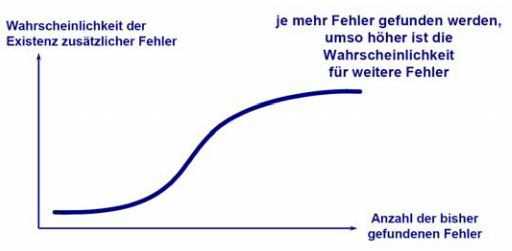
\includegraphics{Figures/error}}
\end{figure}


\subsection{Testen versus Debugging}
Ziel von Testen: \\
Aufzeigen, beweisen, dass Fehler (Bugs) 
existieren --> Destruktives Testen \\
"Jeder gefundene Bug ist ein Gold-Nugget!"

Ziel von Debugging: \\
Die durch Testen gefundenen Bugs beseitigen

\subsection{Laufversuch versus systematischer Test}
Laufversuch
\begin{itemize}
	\item Entwickler testet Code während Implementation 
	fortlaufend
	\item Kann mittels Debugging festgestellt werden
	\item Fehler werden sofort korrigiert
\end{itemize}
	Ist wichtig um zu überprüfen, ob das Programm 
das tut was man will

Systematischer Test
\begin{itemize}
	\item Systematische Fehlersuche
	\item Test werden geplant
	\item SOLL wird mit IST verglichen
	\item Resultate  werden festgehalten
	\item Wenn möglich nicht durch Entwickler der 
	Software
\end{itemize}
Ist wichtig um die Richtigkeit einer Software 
jederzeit reproduzieren und nachvollziehen zu 
können

\subsection{Testarten}

\textbf{Abnahmetest} (Anforderungen; Kunde): Validierung, Besondere Test-Form, Soll nicht Fehler aufzeigen, sondern zeigen, dass das System nach Anforderungen
(gemäss Pflichtenheft) fehlerfrei funktioniert \\
\textbf{Systemtest (Architektur; Tester):} Test des gesamten Systems (z.B. inkl. Mechanik) \\ \textbf{Integrationstest (Entwurf; Entwickler/Tester):} Integration von Programmeinheiten \\
\textbf{Modultest (Detailentwurf/Implementation; Entwickler):} Unit-Test

Die Tests sollten entsprechend den verschiedenen Phasen gemacht werden (Phase und Aktor in Klammern geschrieben). 

\subsection{Verifikation und Validierung}
 Validierung  (Validation)
"Are we building the right product?"
Überprüft das Software-Produkt,
ob es die Anforderungen des Auftraggebers erfüllt.

Verifikation (Verification): 
"Are we building the product right?"
Überprüft die Artifacts während der Entwicklung,
ob sie ihre Vorgaben erfüllen
(Artifacts = künstliche, d.h. von Menschenhand geschaffene Dinge wie Dokumente etc.)

\subsection{Prinzipieller Ablauf eines Tests}
\begin{multicols}{2}
	\adjustbox{width=0.35\textwidth}{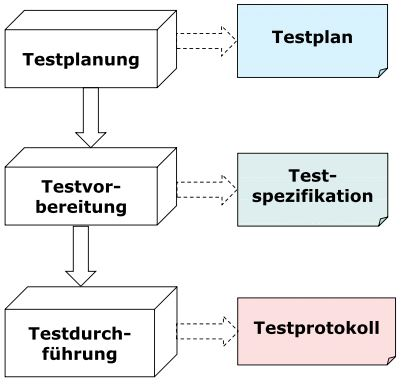
\includegraphics{Figures/testplan}}
\columnbreak

Vorzüge von einem Testablauf: 
\begin{itemize}
	\item  Reproduzierbar
	 \item Wissen, was getestet wurde
	\item Unabhängig von testender Person
	\item Wenn möglich automatisiert
	\item Testspezifikation fortlaufend erweitern
\end{itemize}
\end{multicols}
\subsection{Testspezifikation / Testprotokoll}
Redundanz vermeiden; Möglichst in Code integrieren oder/und 
automatisieren

Elemente: \\
Test-Spezifikation (Test-Code) \\
Test-Protokoll: Wird typischerweise von Test-Frameworks 
erstellt \\
Test-Dokumentation (z.B. mit Hilfe von Doxygen)

\subsection{Auswahl der Testfälle}
Mit den Testfällen die Anforderungen überprüfen
Ziel: Mit möglichst wenig Testfällen möglichst viele Fehler finden

\textbf{Testmethoden: }
\begin{itemize}
	\item Black-Box Testing
	\item White-Box / Glass-Box Testing
\end{itemize}

	\adjustbox{width=\textwidth}{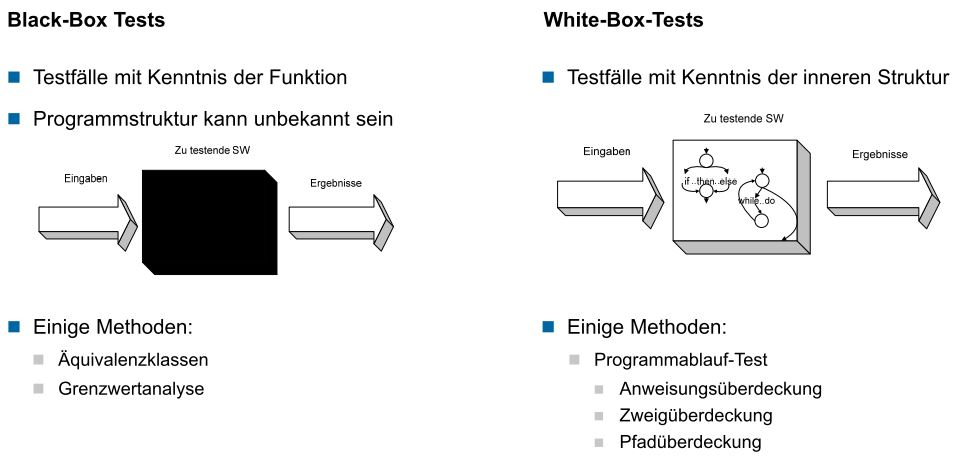
\includegraphics{Figures/blackwhite}}
	
\section{BlackBox Testing}

\subsection{Äquivalenzklassenanalyse}
Äquivalenzklasse = Wertebereich einer 
Eingabegrösse, für welche der Prüfling 
voraussichtlich das gleiche Verhalten zeigt.
Ist Korrektheit der Eingabegrössen nicht 
gesichert auch Äquivalenzklassen für ungültige 
Wertebereiche.

ein Testfall pro Äquivalenzklasse \\
Wert für Testfall kann zufällig sein

\subsection{Grenzwertanalyse}

Erfahrung: Fehler sehr oft an Grenzen 
zulässiger Eingabewertebereiche 
Grenzwertanalyse wählt Testfälle an den 
Grenzen
Werte auf Grenze, knapp darunter und 
darüber.
Kann Äquivalenzklassenmethode erweitern

\subsection{Vergleich} 

	\adjustbox{width=0.8\textwidth}{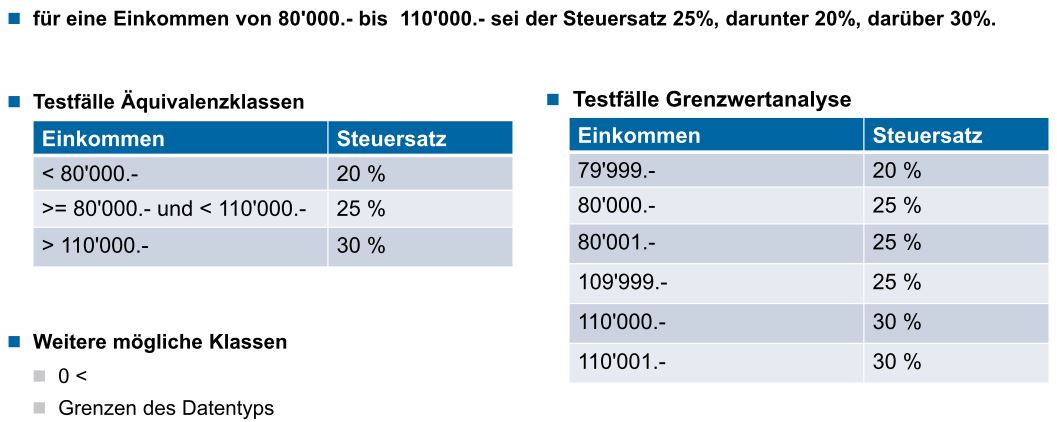
\includegraphics{Figures/vergleich}}
	
\section{White Box / Glass Box Testing}

Kenntnis der Kontrollstrukturen als Basis für Testfälle (Kontrollflussgraph). Jedes Statement als Knoten bzw. sequentielle zu einem Knoten zusammenfassen. Kanten verbinden Knoten entsprechend Verzweigungen und Schleifen.

\adjustbox{width=0.8\textwidth}{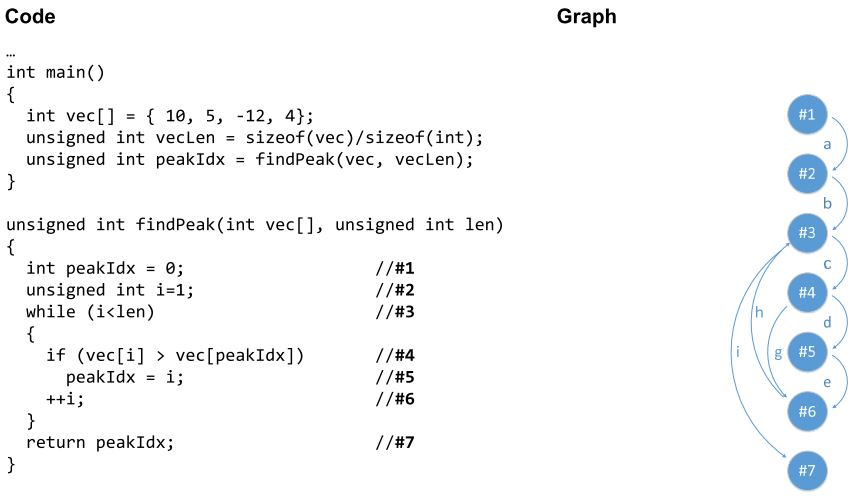
\includegraphics{Figures/kontrollflussgraph}}

\subsection{Anweisungsüberdeckung (Statement Coverage)}
Prozentualer Anteil der Anweisungen, die in 
Test ausgeführt werden 100\% Anweisungsüberdeckung ist Minimum
Alle Knoten werden genau einmal durchlaufen.

Testfälle:
1. int vec[] = {1, 10};

\subsection{Zweigüberdeckung}
 Zweigüberdeckung (branch coverage)
Prozentualer Anteil der Kanten (Zweige), die 
in Test durchlaufen werden
Eine 100\% Zweigüberdeckung enthält auch 
eine 100\% Anweisungsüberdeckung
Zusätzlich werden auch alle "leeren Zweige" 
durchlaufen

Testfälle:
1. int vec[] = {1, 10, 2};
Ablauf: abcde - zurück auf mit i 3-4g - zurück auf 3 i

\subsection{Pfadüberdeckung (Path Coverage)}
Prozentualer Anteil der Pfade, die in Test 
durchlaufen werden
Ein Pfad ist ein möglicher Weg durch den 
Kontrollgraph
100\% Pfadüberdeckung kaum zu erreichen
Die findPeak Funktion kann mit unendlichem 
Speicher unendlich viele Pfade besitzen

Testfälle:
1. int vec[] = {1, 10}; \\
 a, b, c, d, e, h, i \\
2. int vec[] = {1, 10, 2}; \\
 a, b, c, d, e, h, c, g, h, i \\
3. int vec[] = {1, 10, 2, … }; \\

\subsection{Güte}
Die Testgüte hängt von gewählter Überdeckung und erreichtem Überdeckungsgrad ab
Überdeckungsgrad – Prozentuales Verhältnis der Anzahl überdeckter Elemente zur Anzahl vorhandener 
Elemente
Beispiel Anwendungsüberdeckung
int vec[] = { 1 };

\subsection{Greybox-Testing: Pragmatisches Testen}
\begin{enumerate}
	\item Zuerst Black-Box Test
	\item Überprüfung der Anweisungsüberdeckung / Coverage
	\item Ergänzen mittels White-Box Test
	\item Falls gewünschte Coverage nicht erreicht, zum zweiten Schritt springen
\end{enumerate}

Die Kombination von Black- und Whitebox-Testing wird auch Greybox-Testing genannt und wird in der Praxis häufig angewendet.

\subsection{Wann wird welche Testmethode verwendet}

\begin{figure}[hb]
	\centering
	\adjustbox{width=0.7\textwidth}{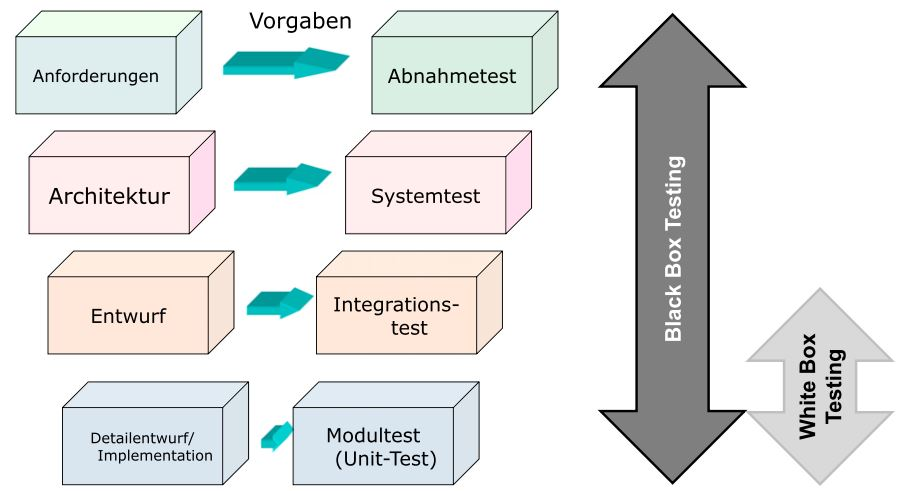
\includegraphics{Figures/testarten}}
\end{figure}


\section{Teststrukturen}

\subsection{Testgeschirr}

Zum Testen unvollständiger Software wird ein Testgeschirr (testharness) benötigt
- wird für das isolierte Testen von Units und Integrationstests benutzt \\
- unabhängig von der Vollständigkeit der Software \\

Ein Testgeschirr besteht aus: \\
- Test-Driver: Ruft den Prüfling auf und Versorgt den Prüfling mit Daten und Nimmt Resultate entgegen und protokolliert sie \\
- Test-Double: berechnet oder simuliert die Ergebnisse einer vom Prüfling aufgerufenen Operation. Kann Mock, Stub, Dummy oder Spy unterteilt werden, haben jedoch keine eindeutige Definitionen. Wir verwenden im allgemeinen den Begriff Mock \\

\begin{figure}
	\centering
	\adjustbox{width=0.7\textwidth}{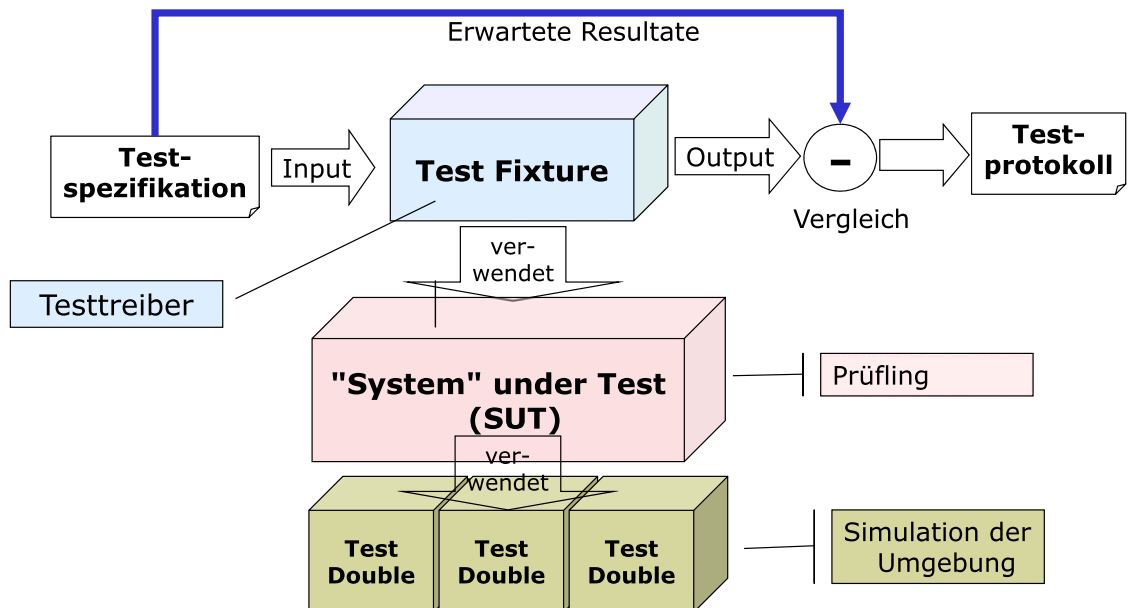
\includegraphics{Figures/testumgebung}}
\end{figure}

\textbf{Testarten} \\

\textbf{Unit-/Komponenten-Tests} bezeichnen das isolierte Testen von Programmeinheiten (Unit = Modul = Methode, Klasse, Komponente) oder mehreren Klassen. Sie sollten gut wiederholbar sein. Die gesamte Umgebung einer Komponente muss durch Treiber und Stümpfe simuliert werden. \\
\textbf{Integrationstest} wird angewendet, wenn ein System schrittweise zusammengebaut wird. Dabei wird die Funktionalität der Baugruppen durch Tests überprüft.  Dabei werden die noch nicht integrierten Teile durch Treiber und Stümpfe simuliert. \\ 
\begin{multicols}{2}
\textbf{Aufwärtsintegration (bottom-up)}\\
- beginnt mit elementaren Komponenten\\
- braucht keine Stümpfe, dafür Treiber \\
\adjustbox{width=0.49\textwidth}{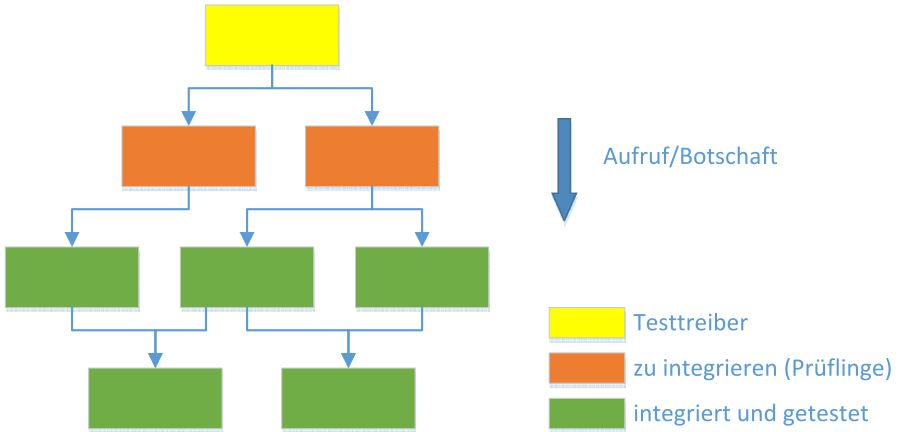
\includegraphics{Figures/aufwaertstest}}
\columnbreak
\\
\textbf{Abwärtsintegration (top-down)}: \\
 - beginnt mit einem "hohlen" Gesamtsystem \\
 -  braucht keine Treiber, dafür Stümpfe
\adjustbox{width=0.49\textwidth}{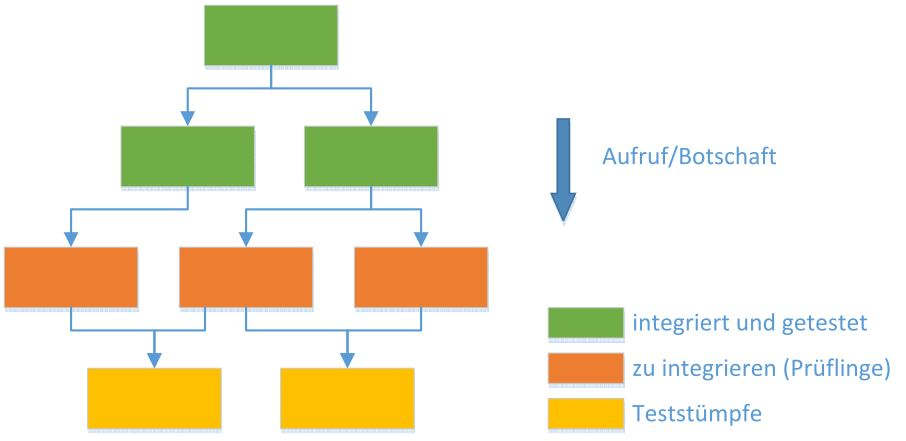
\includegraphics{Figures/abwaertstest}}
\end{multicols}
Mischformen sind ebenfalls möglich. 

\newpage

\begin{multicols}{2}
class A \% \textit{Buch-Klasse} \\
\{ \\
public \\
	A() \\
	\{ b; \\ 
	\} \\
private: \\
B b; 
\} \\

class B \% \textit{Author-Klasse} \\
\{public: \\
private:\\
\} \\

main \\
\{
A a;

\}
\columnbreak

class A  \% \textit{Buch-Klasse} \\
{
public: \\
A(B \&b): b(b)  \\
\% \textit{Jedes Buch A hat einen Autor B} \\
private: \\
B \&b; \\
}

class B \% \textit{Author-Klasse} \\
\{public: \\
\} \\

main \\
\{
B b; \\
A a(b); 
\} \\
\end{multicols}

\subsection{Beispiel a}
\adjustbox{width=\textwidth}{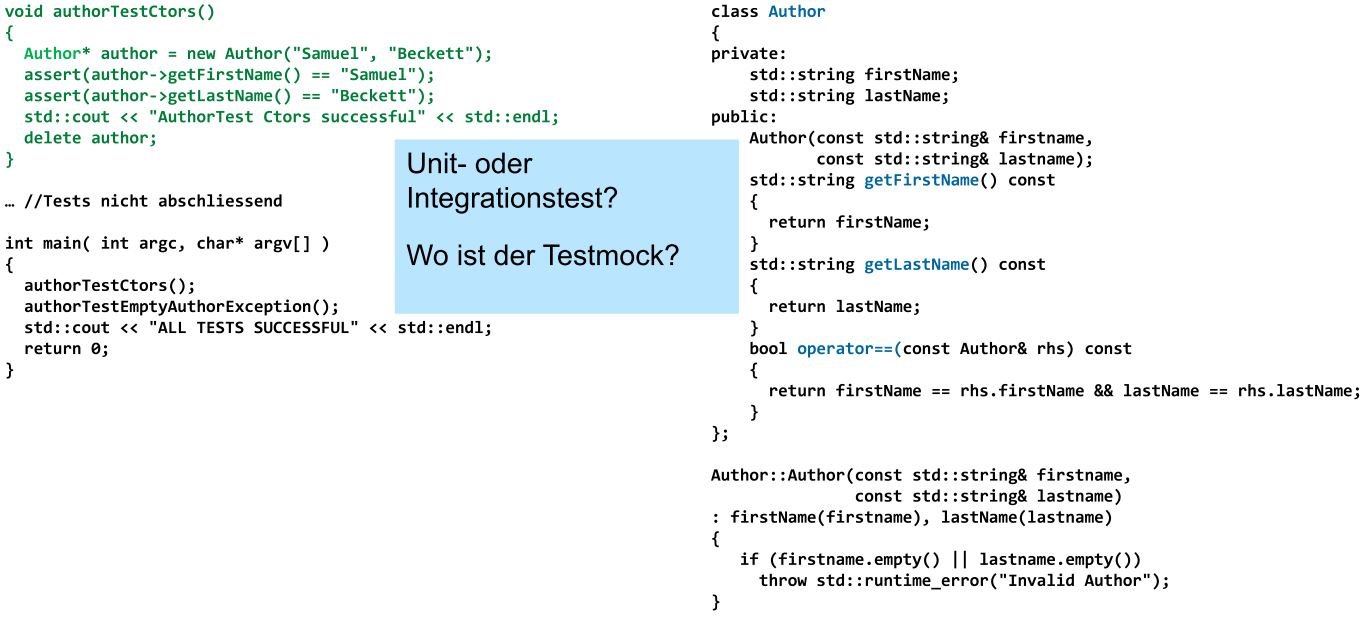
\includegraphics{Figures/beispiela}}
--> Lösung: \\
Unittest (man testet nur diese Klasse); \\
Testmock: Soweit nicht ersichtlich  

\subsection{Beispiel b}
\adjustbox{width=\textwidth}{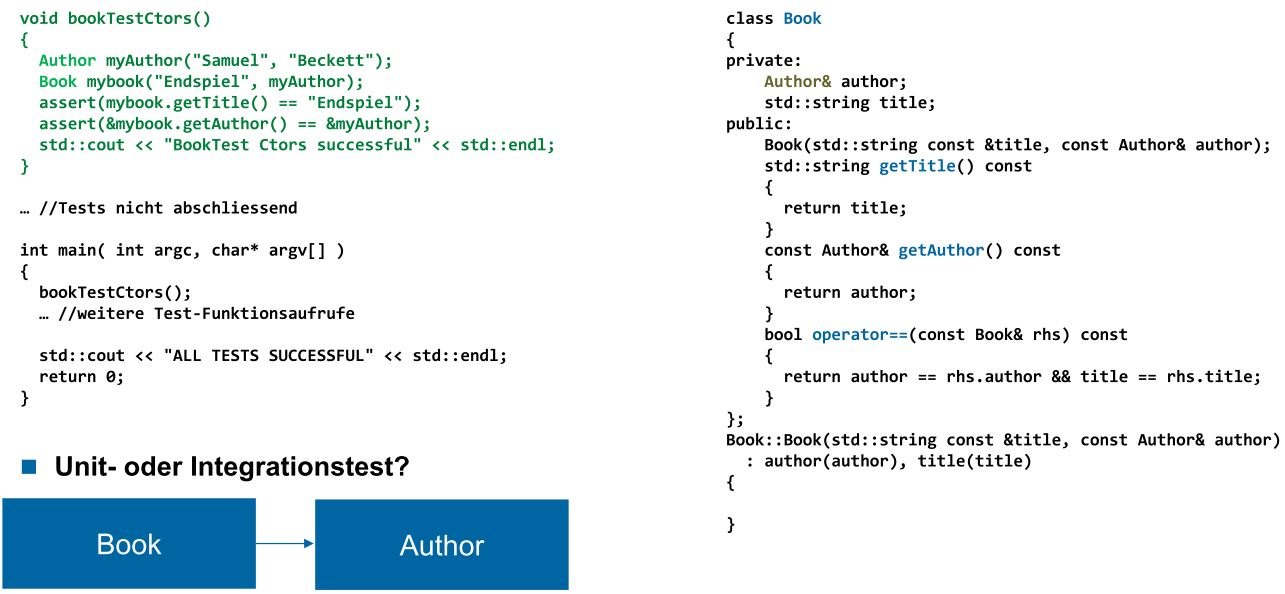
\includegraphics{Figures/beispielb}}
--> Lösung: \\
Integrationstest: Buch und Autor werden miteinander getestet und es wird die Beziehung zwischen Buch und Autor geprüft. 

\subsection{Beispiel c: Dependency Injection}
Pure Virtual Klassen \textbf{müssen} von den Unterklassen überschrieben werden \\
\adjustbox{width=0.9\textwidth}{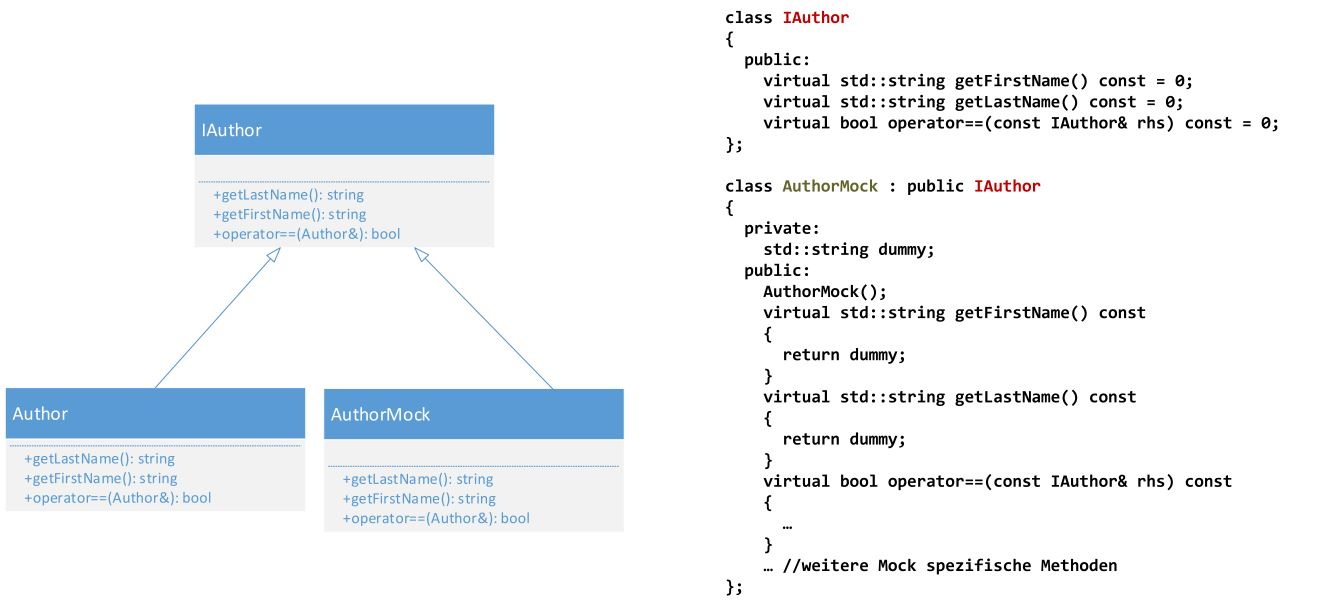
\includegraphics{Figures/beispielc}} \\
\adjustbox{width=0.9\textwidth}{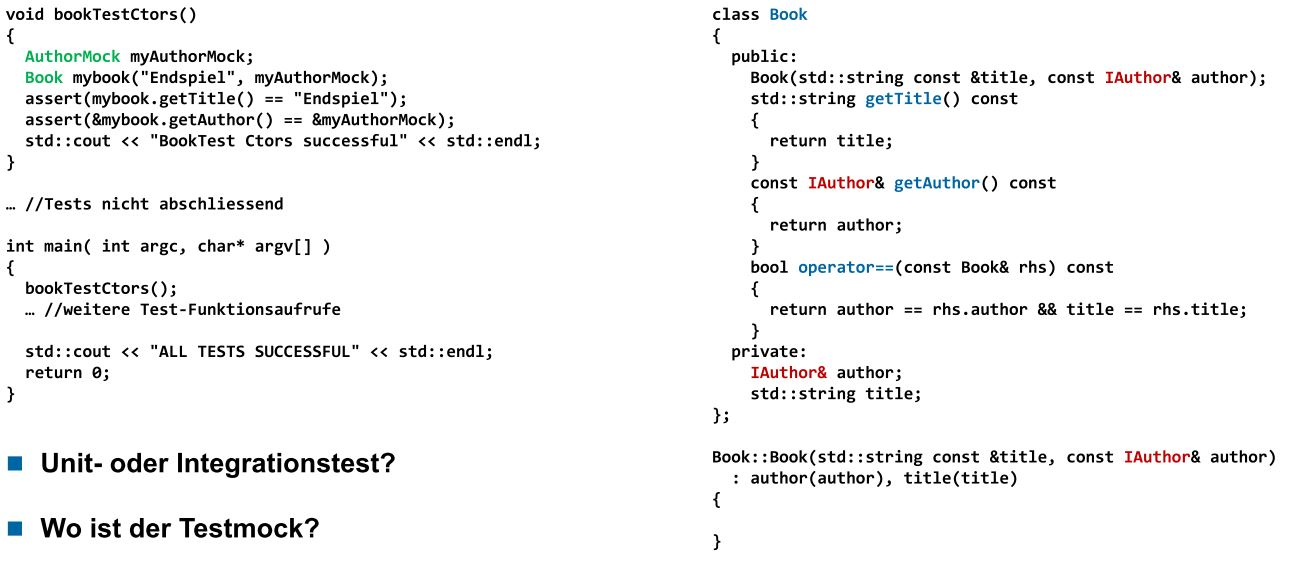
\includegraphics{Figures/beispielc2}}
Nun kann die richtige Klasse oder die Testklasse überprüft werden. \\
Will man Buch testen, kann der Testmock verwendet werden --> Unittest von Buch \\
Die Abhängigkeit zwischen Buch und Autor wurde gelöst. 
Falls nun Autor verändert wird, so kann mit dem "fake Autor" Testmock Author gearbeitet wird. \\
Testmock: AuthorMock (Testklasse für Author)

\subsection{Wann ist genug getestet?}
 Wenn mit den in der Testvorschrift festgelegten Testdatensätzen keine Fehler mehr gefunden 
werden
- Sinnvolles Kriterium, wenn der Umfang des Prüflings eine systematische Auswahl von Testfällen mit 
ausreichender Überdeckung ermöglicht
- Übliches Kriterium bei der Abnahme
- Wenn die Prüfkosten pro entdecktem Fehler eine im Voraus festgelegte Grenze überschreiten
- Sinnvolles Kriterium für das Beenden des Systemtests
- Setzt die Erfassung der Prüfkosten und der Anzahl gefundener Fehler voraus

\section{Automatisierte Tests}
\begin{multicols}{2}
Vorteile: \\
- Wiederholbarkeit \\
- Absicherung bei Änderung, Portierung, Erweiterung \\
- geringe/keine Kosten bei Wiederholung  \\
- Eindeutige Spezifikation \\
- Testcode ist Programmcode und damit eindeutig \\
	\columnbreak
	\\
Nachteile: \\
- Mehr Code zu schreiben und zu pflegen \\
-Testcode ist Programmcode \\
- Werden wirklich die richtigen Anforderungen getestet? \\
- Was muss überhaupt getestet werden? \\
\end{multicols}


\adjustbox{width=0.7\textwidth}{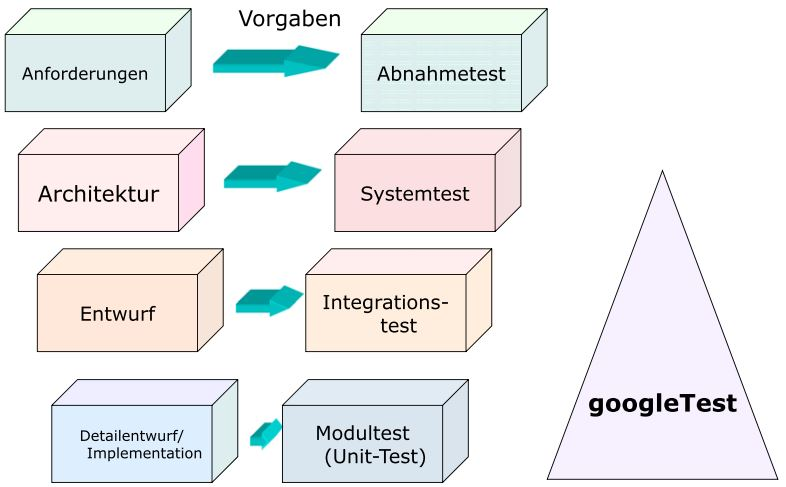
\includegraphics{Figures/werkzeuge}}

\subsection{Unit Test Frameworks}
Um die automatisierten Test zu vereinfachen, gibt es verschiedene Unit Test Frameworks. \\
Bekannte C++ Vertreter sind: googleTest, Boost Test, Qt Test und CppUnit

\textbf{Vorteile von Unit-Testframeworks} \\
- Testfunktionen werden automatisch aufgerufen \\
- Übersichtliche Organisation der Testfälle \\
- Aufteilung der Tests auf mehrere Dateien in der Regel \\
- Zum Beispiel eine Testklasse pro zu testende Klasse. \\
- Innerhalb der Datei: Organisation der Testfälle in Form von Testfunktionen und Testsuiten \\
- Unterstützung bei Test Doubles \\
- Testprotokolle: Ausgabe der Testergebnisse in verschiedenen Formen möglich \\
- Test result formatter ("Outputter") \\

\textbf{googleTest Beispiel} \\
\adjustbox{width=\textwidth}{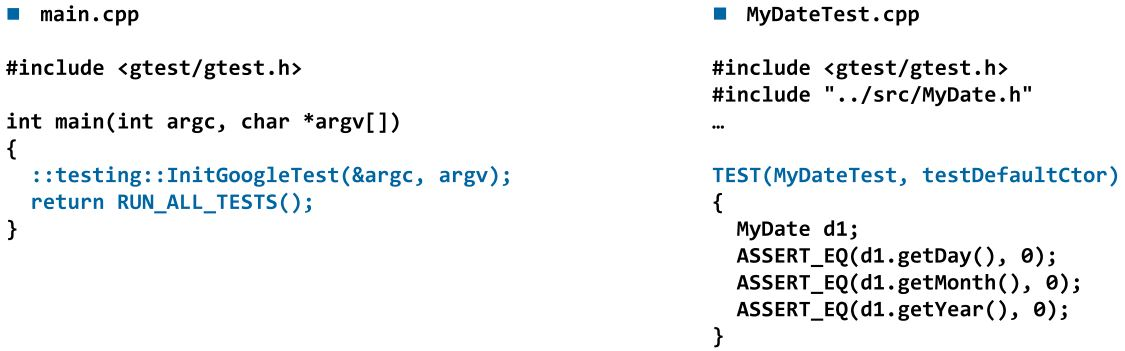
\includegraphics{Figures/googleTest}}

\textbf{googleTest Assertions} \\
- googleTest nutzt selbst definierte Assertions \\
- Beispiele in der Tabelle rechts \\
Weitere Test-Makros können hier gefunden 
werden:
https://github.com/google/googletest/blob/mast
er/googletest/docs/Primer.md

\begin{figure}
	\centering
	\adjustbox{width=0.7\textwidth}{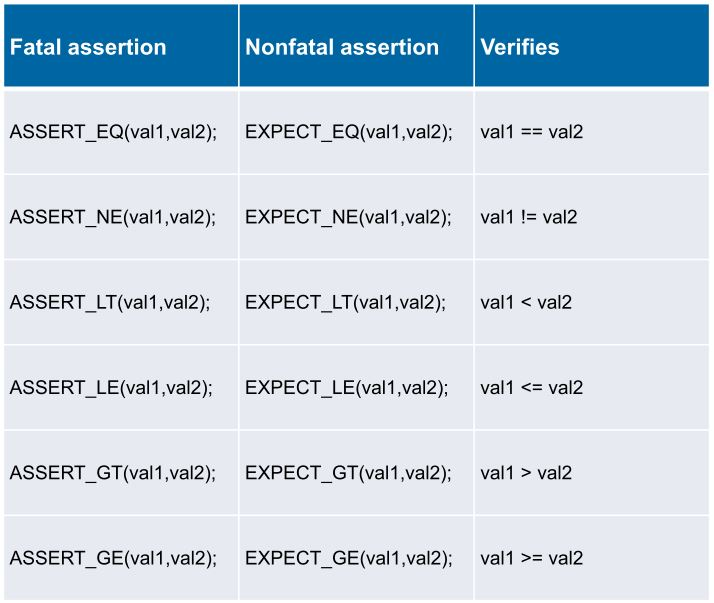
\includegraphics{Figures/assertions}}
\end{figure}


\textbf{Konventionen} \\
 Empfohlene Verzeichnis-Unterteilung
- src Ordner: MyDate.h,  MyDate.cpp, main.cpp \\
- tests Ordner: UnitTest main.cpp, MyDateTest.cpp \\
- Für jede zu testende Klasse wird eine entsprechende Testklasse erstellt.
\textbf{Namensgebung}
- Der Name einer Testklasse beginnt mit dem Namen der zu testenden Klasse und endet mit "Test". Beispiel: Applikations-Klasse "Stack" --> Testklasse "StackTest". \\
- Der Name einer Testfunktion beginnt mit "test": Beispiel: "testAddition()".

\subsection{GCOV Beispiel}
\$ g++ ‐o FindPeak FindPeak.cpp ‐fprofile‐arcs ‐ftest‐coverage \\
\$ ./FindPeak \\
\$ lcov ‐‐capture ‐‐directory . ‐‐output‐file cov.info \\
\$ genhtml ‐‐demangle‐cpp cov.info ‐o html \\
\$ firefox html/index.html \& \\
Wichtig: Flags angeben!

\textbf{Was bedeutet ein Überdeckungsgrad unter 100\%?} \\
- Mit den vorhandenen Testfällen werden nicht alle Anweisungen/Zweige/Pfade ausgeführt \\
- Ist u.a. auch ein Gütemass für die Testfälle \\
\textbf{Massnahmen:} \\
-Zusätzliche Testfälle definieren \\
- Nicht überdeckter Code analysieren, z.B. mittels Code Inspection \\
\textbf{Beim nicht ausgeführten Code kann es sich auch um toten Code handeln} \\
- wenn logisch falsch: korrigieren bzw. entfernen \\
- wenn aufgrund defensivem Programmierstil (z.B. default: break): lassen \\

\subsection{Arten von Tests}

\textbf{Funktionale Tests} \\
gemäss den funktionalen Anforderungen \\
- Testen anhand der vorgestellten Theorie \\
\textbf{Nichtfunktionale Tests} \\
gemäss nicht funktionalen Anforderungen wie Leistungsanforderungen, Leistungstest,  Stresstest, Ressourcenverbrauch, Qualität (wenig ist testbar), Zuverlässigkeit,  Benutzbarkeit, Sicherheit